\section{Previous Work} 
Mainville \& Craymer (2005) used water gauge data collected around the LGL over the past 150 years to
 create monthly means of water level. Differences in these values between sites
 were then plotted against time to calculate a rate of elevation change between
 sites over time (This value is interpreted to represent the impact of the GIA
 process on the crust underlying the LGL, even though the actual process extends
 over a much longer timescale than that of the data collection). Combinations of sites were shown to produce
 inconsistent results, so a second method using a least squares adjustment process was used,
 removing some monthly mean outliers which plotted at or beyond some arbitrary residual distance away 
 from the linear regression line in the vertical (elevation) axis. 
 This process was repeated with each new linear regression on the remaining data
 points until none remained "too far away" from
 the final regression line. A third, and ultimately optimal method for calculating
 GIA was developed by
 Mainville \& Craymer in their 2005 paper, this time computing velocity at a given
 month from the difference between a
 the monthly water level mean and a reference water level for the epoch that the 
 month is found in (this 
 reference level being adjusted for epoch
 and site biases). This elevation difference is then divided by the time difference
 between the start of the epoch and the month that was measured, calculating a rate
 of GIA for the month measured. Their findings with this method showed a general agreement with the post glacial
 ICE-3G global model of GIA at that time, while the ICE-4G model developed by Peltier
 was shown to underestimate the relative difference in vertical movement across
 the span of the Great Lakes (Mainville \& Craymer, 2005).\\ \\
Johnston et al. (2012) attempted to provide a value for GIA in the LGL with
 better accuracy than previous estimates calculated using water
 gauge data.
 
In order to accomplish this, the data used to measure the process of
 GIA needed to extend over a much longer timescale. In this method, water
 levels were inferred from the elevation of relict shorelines in beach ridge
 strandplains from the late Holocene sediment record surrounding Lake Superior.
 Ages for each elevation were inferred from age dating samples from these beach
 deposits (known as strandplain sequences) using
 optically stimulated luminescence (OSL) age dating. Johnston et al (2012) differed from
 Mainville \& Craymer (2005), in that data collected for the 2012 paper using OSL
 age dating did not have
 elevations sampled at the same points in time for calculation of relative
 rates. As a result, Johnston et al (2012) the elevation vs time data was modelled with a linear
 regression for each site, the difference in slopes of each regression representing the GIA rate
 between sites. Individual regressions were further created per site
 for a series of four ranges of time related to lake level phases, namely the Nipissing,
 Algoma, Sault, and Sub-Sault (Johnston et al, 2012). The results reported from this process
 are summarized in Figure \ref{fig:jj2012Grid}. \\
 
 \begin{figure}[t]
	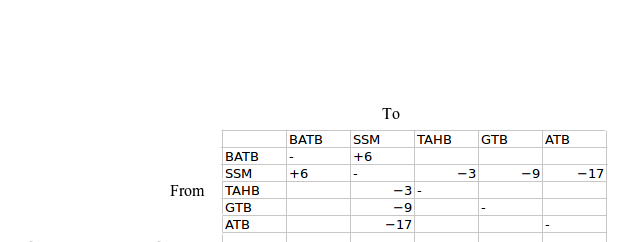
\includegraphics[width=0.9\linewidth]{jjGrid.png}
	\caption{GIA values reported by Johnston et al 2012. All values are reported in cm/century.}
	\label{fig:jj2012Grid}
 \end{figure}
 % need to ask JJ about JJ 2012, bottom of page 3, divergence of intercepts
 
